\section{Dữ liệu}

% ── Slide 1: Nguồn dữ liệu ───────────────────────────────────────────────────
\begin{frame}{Nguồn dữ liệu và gán nhãn}

\begin{columns}[T]
\begin{column}{0.55\textwidth}
  \textbf{Thu thập}
  \begin{itemize}
    \item Crawl video giao thông Việt Nam từ YouTube/web
    \item \texttt{yt-dlp} tải video, OpenCV trích frame
    \item LLaVA lọc frame có dấu hiệu vi phạm
  \end{itemize}
  \vspace{0.4em}
  \textbf{Gán nhãn (bán tự động)}
  \begin{itemize}
    \item \textbf{Grounding DINO} -- tạo nhãn sơ bộ nhanh
    \item \textbf{CVAT} -- hiệu chỉnh \& kiểm tra thủ công
    \item Lưu trữ theo chuẩn \textbf{COCO JSON}
  \end{itemize}
\end{column}
\begin{column}{0.42\textwidth}
  \begin{block}{3 lớp nhãn}
    \begin{itemize}
      \item \texttt{motorbike}
      \item \texttt{helmet}
      \item \texttt{non-helmet}
    \end{itemize}
  \end{block}
\end{column}
\end{columns}

\end{frame}

% ── Slide 2: Tiền xử lý ──────────────────────────────────────────────────────
\begin{frame}{Tiền xử lý và chia tập dữ liệu}

\begin{columns}[T]
\begin{column}{0.55\textwidth}
  \textbf{Chia tập 70 / 10 / 20}

  \vspace{0.3em}
  \begin{table}
  \scriptsize
  \begin{tabular}{lrrr}
    \toprule
    \textbf{Tập} & \textbf{Ảnh} & \textbf{Tỷ lệ} & \textbf{Vai trò} \\
    \midrule
    Train      & 2309 & 70\% & Cập nhật trọng số \\
    Validation & 330  & 10\% & Chọn checkpoint  \\
    Test       & 659  & 20\% & Đánh giá cuối    \\
    \bottomrule
  \end{tabular}
  \end{table}

  \vspace{0.4em}
  \textbf{Tiền xử lý chính}
  \begin{itemize}
    \item Resize ảnh về \textbf{640×640}
    \item Chuyển COCO $\to$ định dạng YOLO
    \item Bổ sung \textbf{pseudo-labels} vào train set
  \end{itemize}
\end{column}
\begin{column}{0.42\textwidth}
  \textbf{Augmentation}
  \begin{itemize}
    \item HSV shift, flip, scale, mosaic (YOLO \& RT-DETR)
    \item Faster R-CNN: không augment mạnh
  \end{itemize}
  \vspace{0.4em}
  \begin{alertblock}{Thách thức}
    Mất cân bằng lớp:\\
    \textit{helmet} $\gg$ \textit{non-helmet}
  \end{alertblock}
\end{column}
\end{columns}

\end{frame}

% ── Slide 3: EDA ─────────────────────────────────────────────────────────────
\begin{frame}{Phân tích dữ liệu (EDA)}

\begin{columns}[T]
\begin{column}{0.48\textwidth}
  \textbf{Phân bố nhãn}

  \vspace{0.3em}
  \begin{table}
  \scriptsize
  \begin{tabular}{lrrr}
    \toprule
    \textbf{Lớp} & \textbf{Train} & \textbf{Val} & \textbf{Test} \\
    \midrule
    motorbike  & 3408 & 906 & 467 \\
    helmet     & 6739 & 450 & 1256 \\
    non-helmet &  900 & 533 & 138 \\
    \bottomrule
  \end{tabular}
  \end{table}

  \vspace{0.2em}
  \centering
  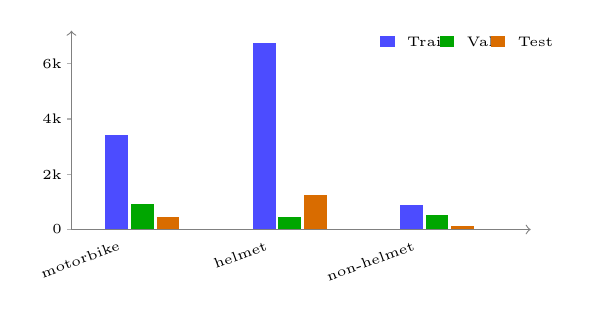
\begin{tikzpicture}[x=0.36cm,y=0.00035cm]
    \draw[->,gray] (0,0) -- (0,7200);
    \draw[->,gray] (0,0) -- (16.2,0);
    \foreach \y/\label in {0/0,2000/2k,4000/4k,6000/6k}
      \draw[gray!60] (-0.15,\y) -- (0,\y) node[left,black] {\tiny \label};
    \foreach \x/\name in {2/motorbike,7.2/helmet,12.4/non-helmet}
      \node[rotate=20,anchor=east] at (\x,-450) {\tiny \name};
    \fill[blue!70] (1.2,0) rectangle (2.0,3408);
    \fill[green!65!black] (2.1,0) rectangle (2.9,906);
    \fill[orange!85!black] (3.0,0) rectangle (3.8,467);
    \fill[blue!70] (6.4,0) rectangle (7.2,6739);
    \fill[green!65!black] (7.3,0) rectangle (8.1,450);
    \fill[orange!85!black] (8.2,0) rectangle (9.0,1256);
    \fill[blue!70] (11.6,0) rectangle (12.4,900);
    \fill[green!65!black] (12.5,0) rectangle (13.3,533);
    \fill[orange!85!black] (13.4,0) rectangle (14.2,138);
    \fill[blue!70] (10.9,6600) rectangle (11.4,7000);
    \node[right] at (11.5,6800) {\tiny Train};
    \fill[green!65!black] (13.0,6600) rectangle (13.5,7000);
    \node[right] at (13.6,6800) {\tiny Val};
    \fill[orange!85!black] (14.8,6600) rectangle (15.3,7000);
    \node[right] at (15.4,6800) {\tiny Test};
  \end{tikzpicture}
\end{column}
\begin{column}{0.49\textwidth}
  \textbf{Thách thức}
  \begin{itemize}
    \item Vùng đầu nhỏ, mờ, bị che khuất
    \item Ánh sáng và góc chụp đa dạng
    \item Mật độ xe cao, đối tượng bị cắt rìa
  \end{itemize}
\end{column}
\end{columns}

\end{frame}
